
\begin{frame}
\frametitle{Temoa}
	\begin{itemize}
		\item Minimizes the system cost
		\item Meets demand of the specified commodities at each time step (electricity, steam, gasoline, etc)
		\item Meets carbon limits at each time step (optional)
		\begin{itemize}
			\item Good at modeling long scenarios (yearly resolution)
			\item Cannot model transients
		\end{itemize}
		\item Temoa is fast, many iterations are possible.
	\end{itemize}
\end{frame}


\begin{frame}
\frametitle{Current model}

	\begin{figure}[htbp!]
		\begin{center}
			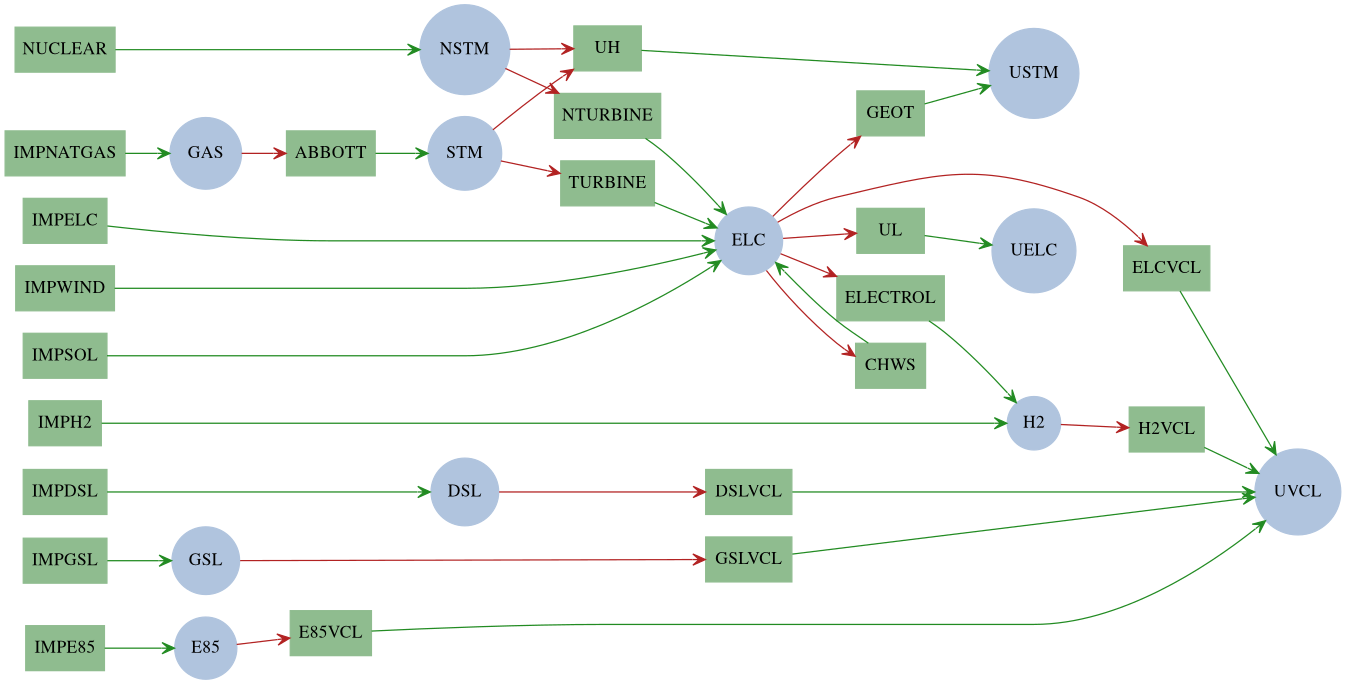
\includegraphics[height=5.6cm]{images/scenario11.png}
		\end{center}
	\end{figure}

\end{frame}


\begin{frame}
\frametitle{Examples of results}

	\begin{columns}
	\column[t]{5cm}
	\begin{figure}[htbp!]
		\begin{center}
			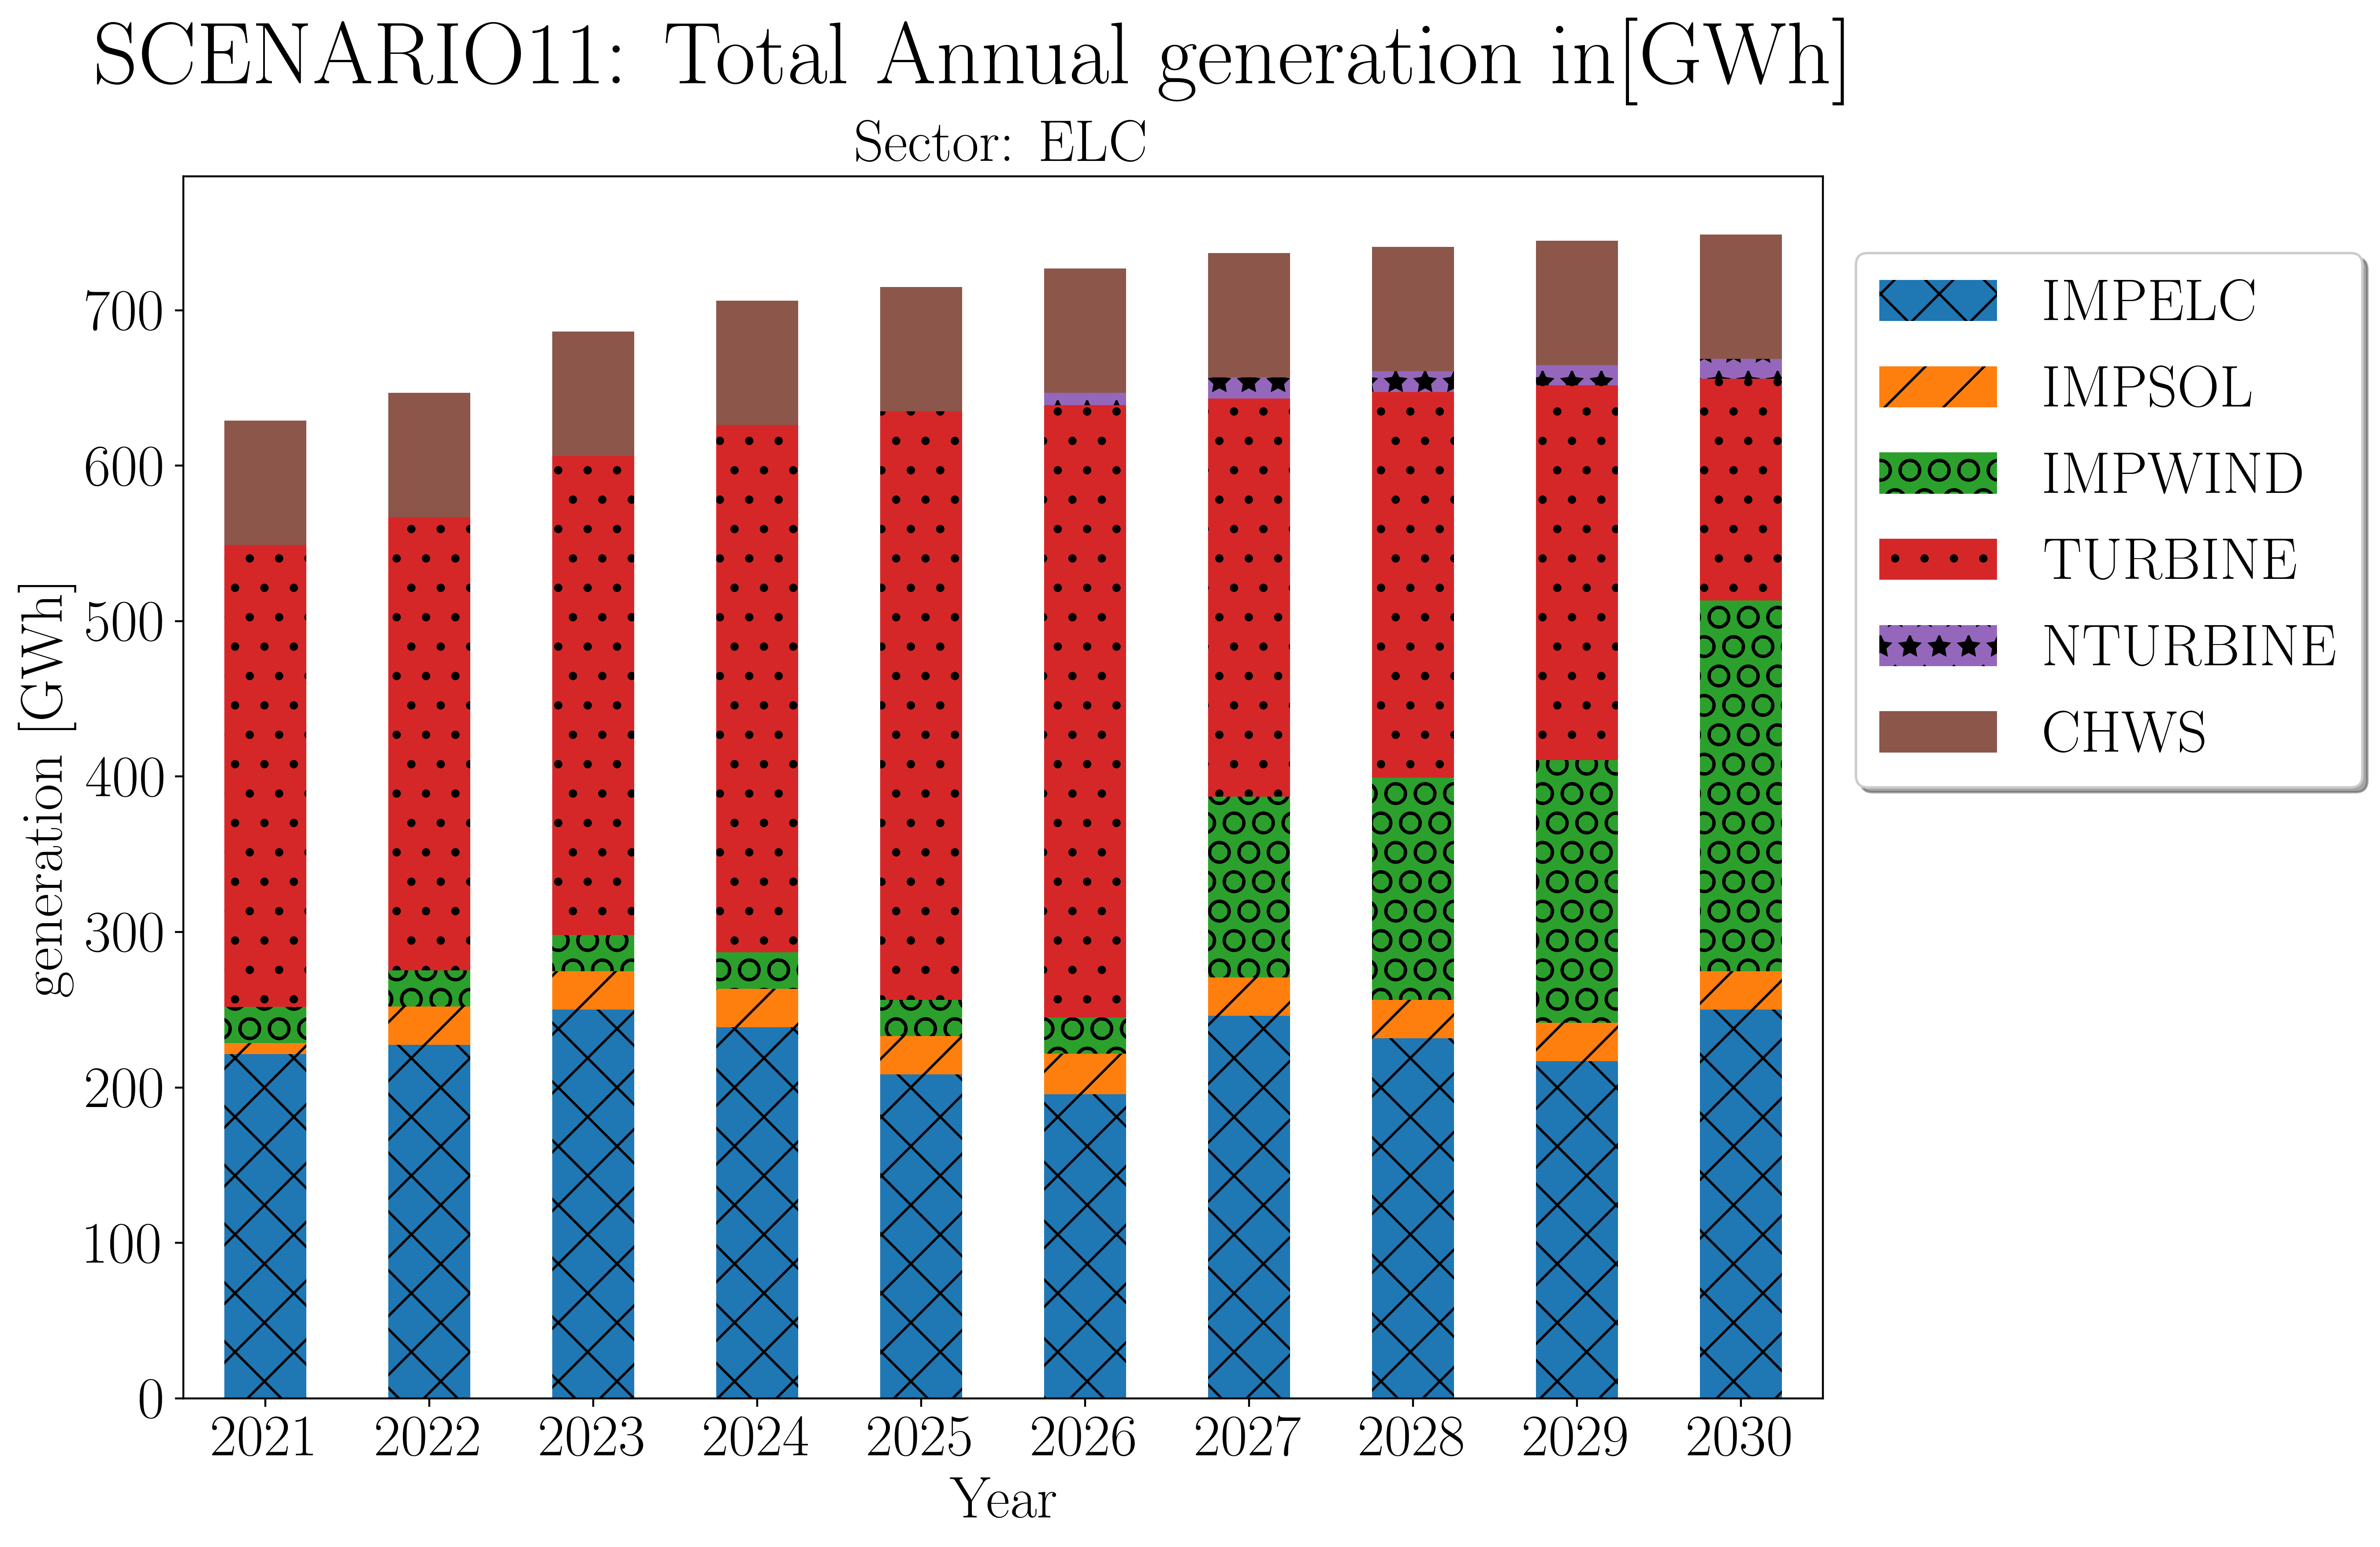
\includegraphics[height=3.8cm]{images/elc-generation.png}
		\end{center}
		\caption{Electricity generated by source.}
	\end{figure}

	\column[t]{5cm}
	\begin{figure}[htbp!]
		\begin{center}
			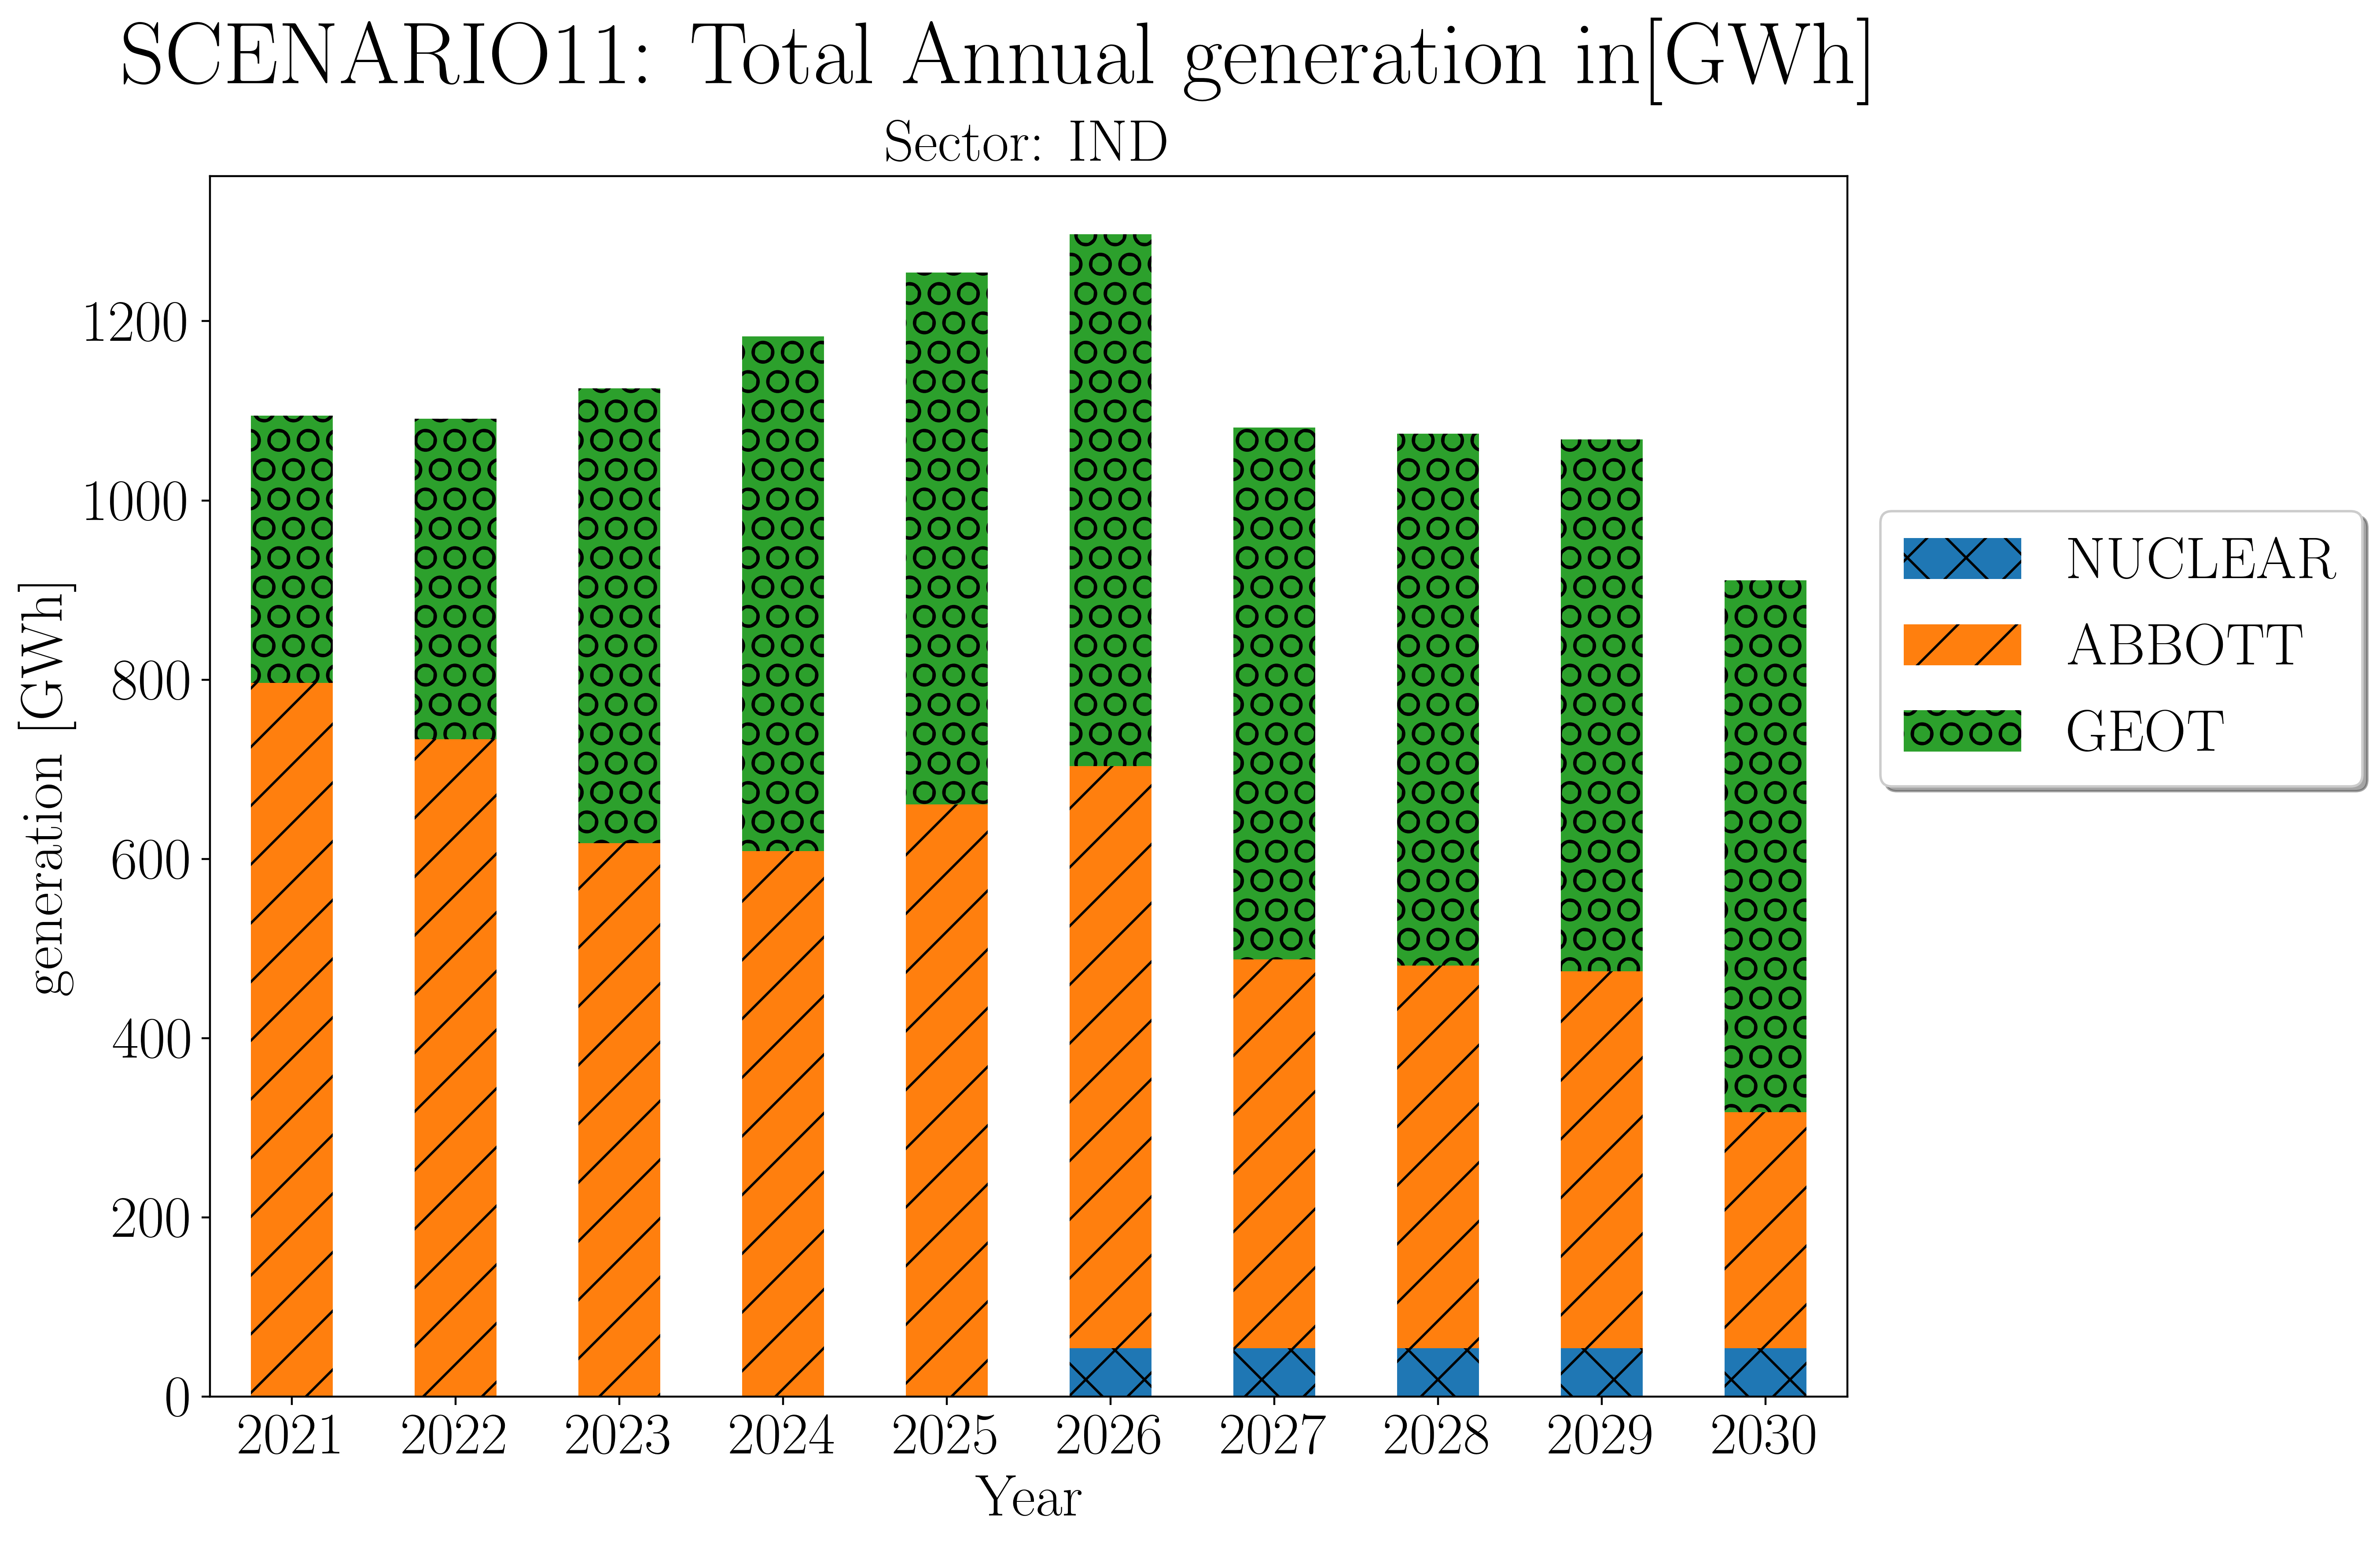
\includegraphics[height=3.8cm]{images/ind-generation.png}
		\end{center}
		\caption{Steam generated by source.}
	\end{figure}
	\end{columns}

\end{frame}


\begin{frame}
\frametitle{Future Tasks}
	Temoa's model:
	\begin{itemize}
		\item Extend current scenario to 2050
		\item Clean Energy Jobs Act: 100\% renewable energy by 2050
		\item Model scenario that minimizes land use with emissions constraints
		\item Create and analyze different possible scenarios. For example:
			\begin{itemize}
				\item with and without Geothermal
				\item with and without alternative vehicles - i.e EVs and FCEVs
			\end{itemize}
	\end{itemize}	

    The bigger picture project:
	\begin{itemize}
		\item Understand Modelica capabilities for modeling the grid
		\item Design integration tool to connect Temoa's results with model in Modelica
		\begin{itemize}
			\item Modelica has Python capabilities (OMPython and PySimulator Package) that could simplify this integration
		\end{itemize}
	\end{itemize}
\end{frame}
